\documentclass[a4paper]{acm_proc_article-sp}  
\usepackage{microtype}
\usepackage{mathpazo}
\usepackage{listings}
\lstset{language=python}
\begin{document}

\title{Fast Response And Intelligently Controlled Harvest Environment}
\author{Peggy Chi \and Jonathan Kummerfeld \and Valkyrie Savage}
\maketitle

\setcounter{page}{1}
\pagenumbering{arabic}

\section{Abstract}

FRAICHE is a complete small-scale sensing and watering system for deployment in community gardens.  The goal is to provide gardeners with a web interface detailing the current status of their plants as well as a machine-learned model of how they ought to care for their plants based on data from their historical plant interactions and the interactions of other gardeners with their plants.  FRAICHE is implemented using a Raspberry Pi, a system with minimal computing power, and we want to leverage this power as effectively as possible to deliver the freshest models to clients when they access the web interface.  In order to effectively test the system, we simulated a scaled up version.  We got RESULTS!

\section{Introduction}

Managing a community garden or small farm is currently a process that requires community members or the farmer to directly monitor their land in an ad-hoc manner.  Additionally, beginning gardeners who lack a large base of knowledge sometimes find it difficult to react effectively to the signals they see coming from their plants, watering them to the point of drowning or failing to notice when they are parched.  Computing has been leveraged to improve the ease of interaction with and analysis of many other physical processes, so we brought machine learning into this challenging gardening environment.

FRAICHE is a system with both sensing and watering capabilities. It can deliver information to the owner about a range of factors, such as moisture and temperature status of the soil around different plants, via a web app.  The same web app allows them to water plants or schedule their watering, with the actual watering accomplished through a configurable drip irrigation system.  Over time, the web app stores data about which plants the gardener waters under which conditions, and will learn how to initiate watering without prompting.  The app also performs machine learning across gardeners: in this way, beginners are able to learn from the experience of those with more established watering practices.

We implemented a complete, small scale system to test computation bottleneck issues for our implementation, particularly for how the sensors being used will manage communication with the central controller. To stress test the system, we simulated a scaled up version. This version involves an extremely large number of sensors working in a star network, with a single central controller receiving data from sensors, constructing/updating models, and handling queries from users.  Constantly asking the sensors for new data and reporting it to various clients is a reasonably simple problem with low overhead, but when running such a system on a machine like the Raspberry Pi that has little computational headroom, balancing the interactions of clients, sensors, and the machine learning tasks becomes a challenge.

In light of this, we tried multiple options for improving response speed.  We implemented several different schedulers to balance the loads of serving clients, getting fresh sensor data, and updating the machine-learned data.  A second option was moving the machine learning task, which was by far the greatest source of CPU use, to the client side in the JavaScript library.  We also implemented a system whereby multiple Raspberry Pis functioning in separate gardens can load balance between themselves via a central data repository.

Following, we describe the several possibilities for balancing serving clients, getting fresh sensor data, and updating the models:

\begin{itemize}

\item Na\"{\i}ve method - each time the server is queried by a gardener, the machine learning algorithm is fed all sensor data and the watering prediction algorithm is updated.

\item Periodic offline computation - according to a schedule, the machine learning algorithm is fed blocks of data containing sensor readings and the prediction algorithm is updated.

\item Sensor-triggered updates - the system reads the sensor data periodically, and when particular events are detected, the machine learning algorithm is given fresh data and started.

\item Hybrid cheap/costly modeling - two different machine learning algorithms are used, one which does "online" computation with all new sensor readings and which is cheap but less accurate, and one which receives batched sensor readings as described above on a periodic basis.  These two models are combined before delivery to the gardner.

\item Updates when load is low - when few clients are connected to and querying sensor readings, a machine learning algorithm update is begun with the stored sensor data.

\item Updates prior to predicted high demand - a second machine learning algorithm observes the typical peaks and valleys in client query traffic, and prior to a predicted peak beings running the machine learning algorithm with fresh data.  This should ensure that the maximum number of clients receive the freshest models.

\end{itemize}

\section{Related Work}

\subsection{Resource Management}

There has been a bevy of work on resource management for both parallel clusters and multiple virtual machines running on a single physical machine.

The Dominant Resource Fairness algorithm \cite{} is designed to help allocate resources fairly in multi-resource systems where processes have heterogeneous demand; it is a port of max-min allocation \cite{} where instead of considering a process's overall needs they are measured as vectors with entries per resource.  However, DRF is designed to work in a system where there are sufficient resources to satisfy all processes' needs, which is different from our situation on the Raspberry Pi.

Jockey \cite{} is another resource management system, and it is built to hold processes to particular Service Level Objectives (SLOs).  Jockey uses predictive algorithms to simulate each job and estimate the time to completion.  FRAICHE differs in that we are aiming to serve models that are as fresh as possible to clients, and the access times of clients are not as well- or strictly defined as SLOs.

Lottery scheduling has been put to use for managing resources: the basic idea is to allot a certain number of tickets to each process requiring a resource based on that process's importance and relative need for the resource.  FRAICHE's goals are not to schedule many processes fairly to run in minimal time, but rather to run the model refinement algorithms as close as possible to clients' requests for plant data.

For virtual machines sharing a physical computer, Xen has explored the resource management question.  However their main challenges lay in isolation of the various virtual machines from each other in order to ensure security, while our challenges lay mainly in scheduling.

Work on scheduling for parallel clusters has included Lithe \cite{}, use of loosely-synchronized clocks \cite{}, and others.  The goal for scheduling with parallel clusters, however, is based mainly on ordering of events when processes don't share a clock.  In contrast, FRAICHE focuses on just one machine on which events take place.

\subsection{Load Balancing}

hardware solutions
software solutions: mechanism of assignment to server
distributed network


\subsection{Machine Learning}

\section{Background}

??????????

\section{Architecture}

FRAICHE is composed of two distinctly different physical systems.  One is the device co-located with plants in the garden.  This device is built on an ATMEL chip.  The second system is a Raspberry Pi, which is located outside the garden.  The two communicate through an XBee wireless radio.

\begin{figure}[h!]
  \centering
    \reflectbox{%
      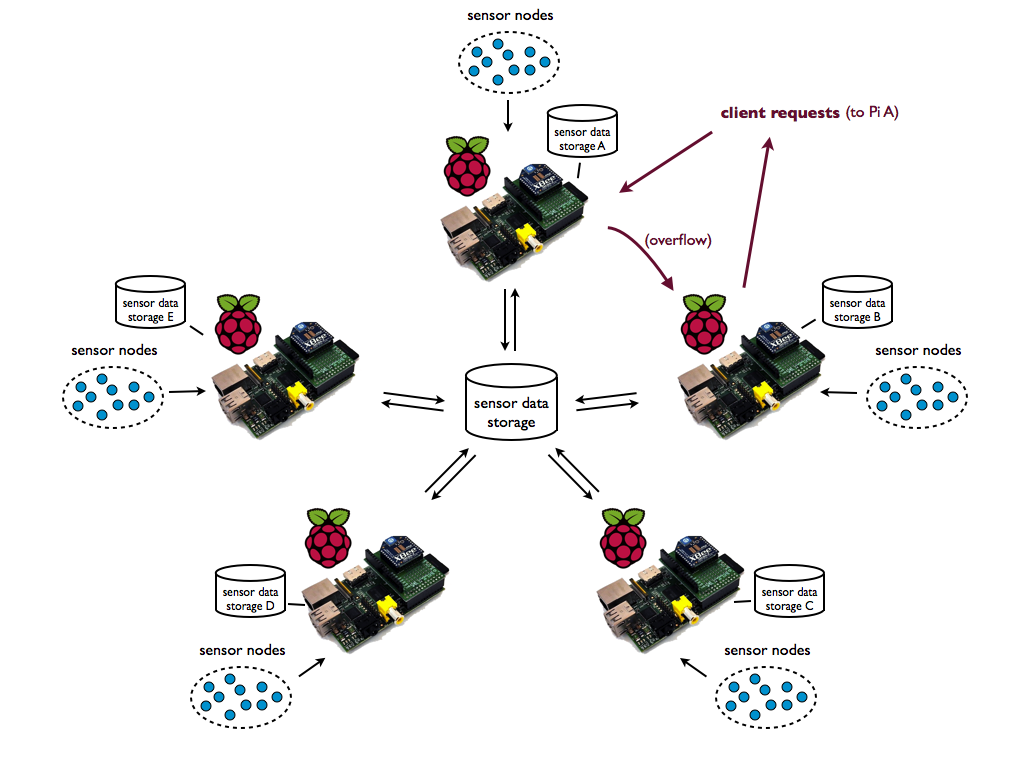
\includegraphics[width=0.5\textwidth]{architecture.png}}
  \caption{Fraiche System Architecture}
\end{figure}

\subsection{In-garden device}

The in-garden device contains several components within a 3D printed body and is connected to a drip irrigation system.  A servo attached to a valve controls the flow of water in the downstream portions of the irrigation system.  This servo is controlled by an ATMEL chip.  Attached to the circuitboard with the ATMEL chip is an XBee radio for communication, an array of sensors for detecting moisture, temperature, etc., of the soil, a battery, and a solar panel.  On the top of the device there are also four buttons for managing watering configurations while co-located with the plants (i.e. the user need not access the website to adjust watering thresholds: he or she can push a few buttons while looking at the plant if it seems to be too dry or too wet).

This device awakens from sleep mode approximately once per hour or when the buttons are pushed.  Whenever it is awake, it begins the communication process described below.

\subsection{Raspberry Pi(s)}

The Rapsberry Pi is a low-cost (~USD35), portable single-board computer released in 2012. In our system, the Raspberry Pi is connected to the Internet and also has an XBee mounted in order to communicate with the in-garden devices.  It serves three purposes: it maintains communication with all in-garden plant systems, it provides a web interface for gardeners to monitor their plants and update their watering configurations, and it maintains models of the typical watering patterns of the plants.

The RPi's communication with the in-garden plant systems takes the form of a very brief exchange initiated by those systems.  Since power consumption is tight on the battery-powered systems, this communication takes place about once per hour.  To differentiate between readings, messages sent by each in-garden device are preceded by that device's unique ID.  When a reading is received by the RPi, it either sends the most recent watering instruction it received from the gardener via the website or a single acknowledgement character.

The Raspberry Pi also runs a simple webserver which allows gardeners to track the measured readings of their plant along with a display of the current machine-learned model.

In the scenario we describe with multiple Raspberry Pis, each has a connection to a central database (stored in the cloud using Amazon EC2 service) which serves as a data repository. The system is designed to be scalable: when a new device connects to the system, it registers with its IP address and the information is broadcasted to the whole gardening distributed network. 

\section{Implementation}

All systems were composed in Python 2.7, and all tests were performed on a Raspberry Pi Model B, running Linux Debian.  Specs of the Raspberry Pi are as follows: 700MHz ARM 1176JZF-S core, Broadcomp VideoCore IV, 512MB SDRAM shared between CPU and GPU, 32GB SD card.  The RPi is rated to 700mA at 3.5W. 

On the client side, the web user interface complies with web standards and runs JavaScript to display the latest data with visual graphs in real-time.

\subsection{Webserver}

We elected to use a pre-made open-source webserver for our implementation: Tornado \cite{}.  It was created by Friendfeed for their primary web stack, and later open sourced by Facebook after their acquisition \cite{}.  Tornado allows for different handlers to be attached to different web addresses.  One of these is the plant data page, which is loaded by each client; one is a WebSockets endpoint, which is connected to by the main page upon loading; and one is a sensor update endpoint for testing.

The plant data page contains a graph, powered by the Google Stocks API, of historical plant water data and also a display of the predicted water model.  It has a form by which the client can send explicit instructions for desired watering specifications to the in-garden device and toggle automatic watering.  The WebSockets connection is created in Javascript when this main page is loaded: the WebSockets pipe is used for transmission of plant and model data to the client and instructions transmission from the client.  The most recent 15 historical data points for plant moisture are transmitted when the page is loaded, afterwards sensor and model data are updated whenever new data are available.

In order to build a test harness which can simulate many sensors and many clients without the need for in-garden devices, our other endpoint is a sensor update endpoint.  From here, we log the data from incoming sensors to a file for later access.  This endpoint also updates the schedulers with information about when new sensor data are available.

\subsection{Schedulers}

Six independent schedulers were built, as described in the Introduction: Na\"{\i}ve, Periodic Offline, Sensor-triggered, Hybrid, Low Load, and Predicted Demand.  The scheduler API is as follows:

\begin{lstlisting}
gotSensorEvent(plant_num, value) # by default, does nothing
gotClientRequest(plant_name) # by default, does nothing
timeToRunML() # returns bool ; by default, returns false
runMLPredict() # returns float
runMLUpdate() # returns float
\end{lstlisting}

\lstinline|gotSensorEvent|, \lstinline|gotClientRequest|, and \lstinline|timeToRunML| are over-riden by subclasses as appropriate.  All subclasses use the default \lstinline|runMLPredict|, which returns a float indicating the predicted soil moisture at the next time step, and the default \lstinline|runMLUpdate|, which feeds all not-yet-used sensor date to the model.

The server calls \lstinline|gotSensorEvent| and \lstinline|gotClientRequest| when it gets appropriate events and before it handles them internally.  A periodic callback is implemented to ping the scheduler every 5 seconds querying whether it needs to run its ML algorithm.  This is important for the scheduling algorithms that do not have event-based model updates.

\subsubsection{Na\"{i}ve Scheduler}

The na\"{i}ve scheduler is very simple: when its \lstinline|gotClientRequest| function is called, it takes all sensor data not yet incorporated into the model and updates the model with it.  It uses default functionality for the remainder of the functions.

\subsubsection{Periodic Offline Scheduler}

The periodic offline scheduler has a period of 5 minutes.  Once five minutes has elapsed since the last time its model was updated, all new data are fed to the model.

\subsubsection{Sensor-triggered Scheduler}

The sensor-triggered scheduler overrides \lstinline|gotSensorEvent| to update the model after each sensor reading is recorded.

\subsubsection{Hybrid Scheduler}

The hybrid scheduler has an instance of the periodic offline scheduler and an instance of the sensor-triggered scheduler, which each run their own model updates when appropriate.

\subsubsection{Low Load Scheduler}

The low load scheduler defines ``low load'' as fewer than 15 client requests in the preceding 5 minutes.  If this load is seen at one of the periodic callback checkpoints, the model is updated with all fresh sensor data.

\subsubsection{Predicted Demand Scheduler}

The predicted demand scheduler has a meta-scheduler of the na\"{i}ve variety.  This meta scheduler models client request traffic.  When the meta-scheduler reports that client demand is predicted to increase in the near future, the models of plant moisture are updated with all fresh sensor data.

\subsection{Machine Learning Algorithms}

\subsection{Client-side Modeling}

One inspiration from working with Raaspberry Pi is to leverage computation to the clients, while current web browsers and consumer devices are capable to perform reasonably heavy computation. Therefore, we moved the machine learning task, which was by far the greatest source of CPU use, to the client side in the JavaScript library when receiving the data update. In this way, we reduce the workload of the web server at the cost of repetitive client-side computation. We suspect this is a reasonable tradeoff for a low-cost network system.

\subsection{A World of Multiple Pis}

Moving beyond a scenario of , we consider more devices...

We added an additional Raspberry Pi and facilities for the two to communicate and load balance using Amazon Cloud Services as an intermediary data storage location.  This system is scalable and self-balancing.

Report to the central storage: We chose to use the free tier of the Amazon EC2 (Elastic Compute Cloud) service that provides flexible and scalable capacity in the cloud. 

Inter-Pi communication: http requests, web sockets

\subsection{Simulation Harness}

The simulation harness we constructed is also written in Python.  It builds off the splinter \cite{} library which can instantiate multiple full web browsers.  This feature is necessary for measuring the load time accurately: the client's page is only considered to be "loaded" when the 15 most recent historical data points (transmitted via WebSockets, as described above) are found in the page's JavaScript.

Client processes are forked from the main process: each client has a configurable list of plants from which list one plant is chosen randomly to query at each time step.  

\section{Performance}

We simulated three scenarios for FRAICHE: personal garden, community garden, and small farm.  Each of these scenarios has a distinctive balance between clients and plants.  All simulations were performed on the Raspberry Pi with client requests and sensor updates issued from a MacBook Pro.

Client request batches were issued in 15 second time steps.  A sine curve with some noise determined how many clients made fresh requests at each step.

Sensor update batches were also issued in 15 second time steps.  All sensors reported new data at each time step.

\subsection{Personal Garden}

A personal garden is characterized by a single person caring for a small number of plants.  For the purposes of our simulation, we chose 5 to be a small number of plants: this scenario has one client and five plants.

\subsection{Community Garden}

PhantomJS

A community garden is made up of many people tending many plants.  We simulated 50 clients and 100 plants.

\subsection{Small Farm}

A small farm comprises many plants and a single farmer.  For our simulation, we ran one client and 100 plants.

\subsection{Client-side Modeling}

lala

\subsection{Load Balancing Between Pis}

lala
graph of latency here

\section{Conclusions and Future Work}

In the future, we think it would be valuable to explore the space of very small commodity computers further.  There are many open questions relating to their performance for tasks

acquiring real-time weather conditions (e.g. weather.com XML format)

trigger on sensors

compare with other watering systems (ETO)

\bibliography{bib}
\bibliographystyle{plainnat}
\end{document}
